\documentclass[runningheads,a4paper]{llncs}

\usepackage{amssymb}
\setcounter{tocdepth}{3}
\usepackage{graphicx}
\usepackage{subfig}
%\linespread{2}

\usepackage{url}
\usepackage{csquotes}
\newcommand{\keywords}[1]{\par\addvspace\baselineskip
\noindent\keywordname\enspace\ignorespaces#1}

\usepackage{listings}
\usepackage{color}
\usepackage{enumitem}
\usepackage{hyperref}

\definecolor{dkgreen}{rgb}{0,0.6,0}
\definecolor{gray}{rgb}{0.5,0.5,0.5}
\definecolor{mauve}{rgb}{0.58,0,0.82}

\lstset{frame=tb,
  language=C++,
  aboveskip=3mm,
  belowskip=3mm,
  showstringspaces=false,
  columns=flexible,
  basicstyle={\small\ttfamily},
  numbers=left,
  numberstyle=\tiny\color{gray},
  keywordstyle=\color{blue},
  morekeywords={vector},
  commentstyle=\color{dkgreen},
  stringstyle=\color{mauve},
  breaklines=true,
  breakatwhitespace=true,
  tabsize=3
}

\begin{document}

\mainmatter  % start of an individual contribution

% first the title is needed
\title{Menura: \\ Realtime pitch detection in C++}

% a short form should be given in case it is too long for the running head
\titlerunning{menura}

%
\author{Valentina Visintini}
%
\authorrunning{menura}
% (feature abused for this document to repeat the title also on left hand pages)

\institute{Practical Course "Advanced Software Development with Modern C++"\\Summer Term 2018\\Institute for Computer Science\\
Ludwig-Maximilians-Universit\"at M\"unchen\\
}

\maketitle


\section{Introduction}
A typical task of digital signal processing is to identify the pitch of an audio signal. In this project, a whistled audio signal is analyzed to identify the played note in realtime. To achieve this, the programming language C++ was chosen, as it is very efficient and allows for an implementation based on formal concepts.


\section{A Brief Outline of Acoustics}
In music, a \textit{pitch} is the position of a single sound within the complete range of sound, which is perceived according to the frequency of vibration of the sound waves. Human listeners perceive higher frequencies as higher pitches, hence a lower pitch is indicative of a lower frequency.
A pitch detector aims to find the fundamental frequency of an audio signal, i. e. the lowest frequency of a periodic waveform, to determine what note is being played. Since the fundamental is also perceived as the loudest, the ear identifies it as the specific pitch of the musical tone

Sound waves cause a local pressure deviation from the ambient atmospheric pressure, which is known as sound pressure and perceived as \textit{loudness}. Even though it can be ordered on a scale extending from quiet to loud, loudness cannot be measured objectively, as its perception changes individually, whereas the actual sound pressure can be measured using a microphone and expressed in decibel (dB). The sound pressure level $L_p$ is defined by a logarithmic measure of the effective pressure of a sound $p$ relative to the standard reference sound pressure $p_0$ in air or water. 

\begin{equation}
L_p = 20 * \log_{10}(\frac{p}{p_0}) \mathrm{dB}
\label{eq:spl}
\end{equation}

\section{Frequency Spectrum Analysis}
\label{sec:fft}
The fundamental frequency of an audio signal can be obtained by a fast Fourier transform (FFT). This algorithm samples a signal over a period of time and divides it into its frequency components, converting it from the time domain to a representation in the frequency domain.

\begin{equation}
\sum_{n=0}^{N-1}x_n  e^{-i 2 \pi k\sqrt{-1}/N}
\label{eq:fft}
\end{equation}

In order to detect the pitches of an audio signal, it is split up in equal sample windows and each window is analyzed separatedly. The size of the windows, i. e. the FFT size, affects the resolution of the resulting spectra: the larger the size, the higher it is. The frequency resolution $f_{res}$  is equal to the reciprocal of the time window duration $T_{win}$. So for $M$ samples going into the FFT and a sampling period of T seconds, then $T_{win} = M*T$, thus $f_{res} = 1/(M*T)$. $F_s$ is the sampling frequency, with $F_s = 1/T$.
The resulting output contains the magnitude information for the respective frequency at each bin (index) k and can be converted to the frequency this way:

\begin{equation}
f = \frac{k}{M \cdot T} = \frac{k}{M} \cdot {F_s}
\label{eq:fft}
\end{equation}

The magnitude of each FFT bin i can be expressed like this:
\begin{equation}
mag(k) = \sqrt{(re(k)^{2} + im(k)^{2})}
\label{eq:mag}
\end{equation}

To obtain the loudness of each frequency, the magnitude must be transformed to decibel:

\begin{equation}
A(k) = 20 * \log_{10}( mag(k) ) \mathrm{dB}
\label{eq:loc}
\end{equation}

Starting from this, the frequency with the largest magnitude can be identified as the fundamental frequency of the analyzed window.

\section{Matching Frequency to Note}
\label{sec:match}
A note can be matched in many ways but one would be via the corresponding key on a piano. It is calculated by the relation of the frequency to the concert pitch (A4) and the result is the keyboard index of the detected note.

\begin{equation}
d_f = 49 + 12  \cdot \log_2 \left(\frac {f}{440\ \mathrm{Hz}}\right)\,
\end{equation}

Every note has their ideal frequency but, of course, it is not very likely to be met when the audio input is whistling. So there is a range in which a pitch will be accepted as note that can be mathematically expressed by cents.


\begin{equation}
n = 1200 \cdot \log_2 \left( \frac{b}{a} \right)
\end{equation}


\section{Modeling}
To enable an analysis of the frequency spectrum, an audio signal must be converted to a sequence of samples first (see Fig. \ref{fig:sample}). 

\begin{figure}[]
  \centering
  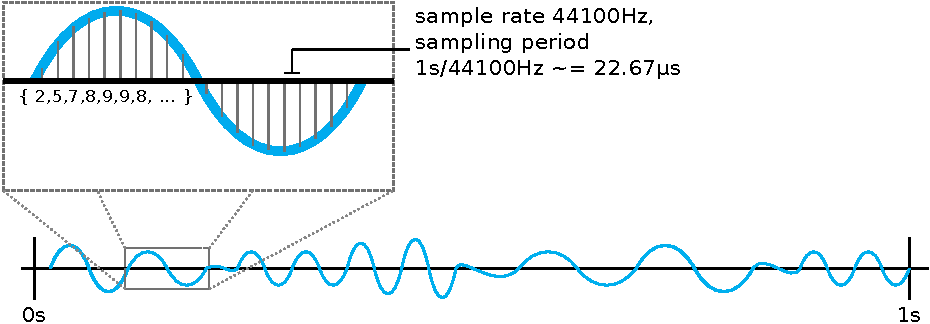
\includegraphics[width=\textwidth]{img/menura_sampling.pdf}
  \caption{Audio sampling}
  \label{fig:sample}
\end{figure}

Now the signal can be split up into sample windows and transformed from time domain to frequency domain, as described in section \ref{sec:fft} (Fig. \ref{fig:fft}.

\textbf{
\begin{figure}[]
  \centering
  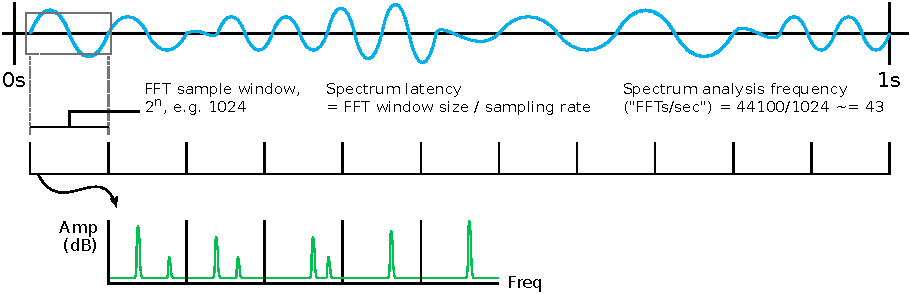
\includegraphics[width=\textwidth]{img/menura_fft.pdf}
  \caption{Frequency Spectrum Analysis \& Signal Transformation: Time Domain to Frequency Domain}
  \label{fig:fft}
\end{figure}
}

In order to find the fundamental frequency, the maximum must be determined by finding the largest magnitude in the spectrum (Fig. \ref{fig:prune}).

\textbf{
\begin{figure}[]
  \centering
  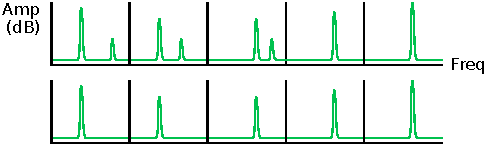
\includegraphics[width=0.5\textwidth]{img/menura_pruning.pdf}
  \caption{Pruning}
  \label{fig:prune}
\end{figure}
}

The last step is to match the frequency to the corresponding note (Fig. \ref{fig:class}), so it can be processed further, e. g. to be written to MIDI.

\textbf{
\begin{figure}[]
  \centering
  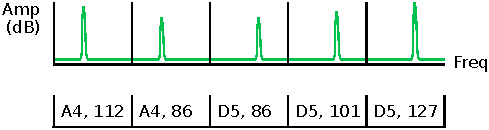
\includegraphics[width=0.5\textwidth]{img/menura_note.pdf}
  \caption{Labeling}
  \label{fig:class}
\end{figure}
}


\section{Implementation}
Menura contains several separate modules as shown in Fig. \ref{fig:sysdia}. The input module handles the audio input stream which is passed to the next module, performing the frequency spectrum analysis. The resulting frequencies are further processed by pruning and the fundamental frequency is selected in order to be labeled a note by the next module. The detected note is then written to the the command line.

\textbf{
\begin{figure}[]
  \centering
  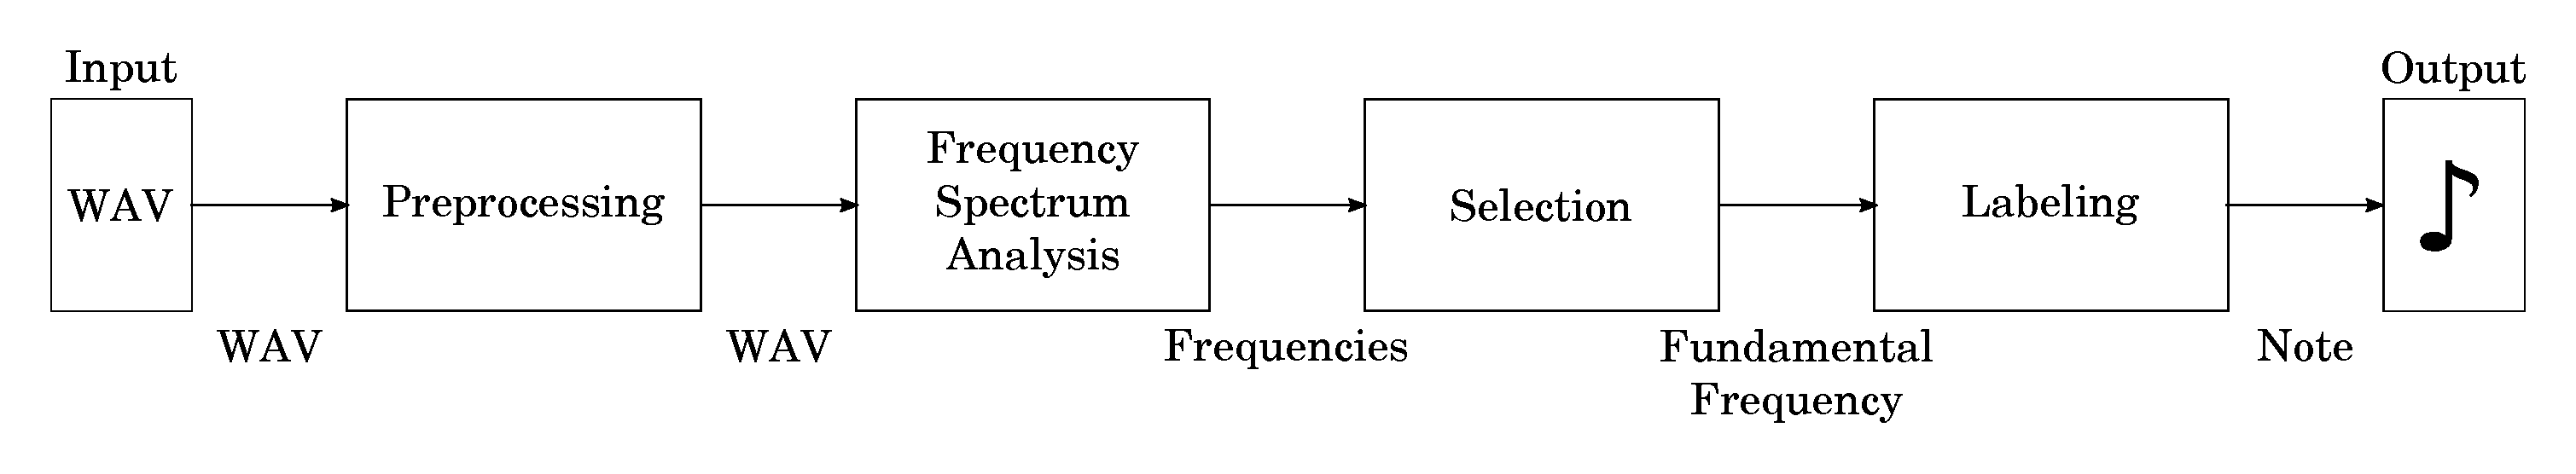
\includegraphics[width=\textwidth]{img/systemdiagram.pdf}
  \caption{System diagram}
  \label{fig:sysdia}
\end{figure}
}

The audio is recorded by means of an asynchronous callback of the PortAudio \cite{port} library, which enables cross-platform realtime audio in- and output. The data written to the input buffer and then passed to the frequency spectrum analysis. For calculating the FFT the FFTW \cite{fftw} library, a C subroutine library for computing the discrete Fourier transform, was used.

The labeling was realized as described in section \ref{sec:match}:

\begin{lstlisting}[caption=Note detection]
note note_of(double frequency, double pitch_hz = 440.0) {

  int note_idx = 12 * std::log2(frequency / pitch_hz) + a4_idx;

  double ideal_freq = pitch_hz * std::pow(2.0, (note_idx - a4_idx) / 12.0);
  
  int cent_idx = 1200 * std::log2(frequency / ideal_freq);

  if(frequency >= ideal_freq) {
    if(cent_idx > 50) {
      note_idx++;
      cent_idx = 100 - cent_idx;
      if(cent_idx != 0)
        cent_idx = (-1) * cent_idx;
    }
  }
  // else analogously
}
\end{lstlisting}
 \label{fig:cents}

The performance of the system depends on the FFT, which is more or less efficient depending on the specified FFT size that can be set at program start. As for the rest, every step of the process is deterministic in both in time and memory, independently of the input.

\bibliography{literature}
\bibliographystyle{plain}

\end{document}
